% Options for packages loaded elsewhere
\PassOptionsToPackage{unicode}{hyperref}
\PassOptionsToPackage{hyphens}{url}
%
\documentclass[
]{article}
\usepackage{amsmath,amssymb}
\usepackage{setspace}
\usepackage{iftex}
\ifPDFTeX
  \usepackage[T1]{fontenc}
  \usepackage[utf8]{inputenc}
  \usepackage{textcomp} % provide euro and other symbols
\else % if luatex or xetex
  \usepackage{unicode-math} % this also loads fontspec
  \defaultfontfeatures{Scale=MatchLowercase}
  \defaultfontfeatures[\rmfamily]{Ligatures=TeX,Scale=1}
\fi
\usepackage{lmodern}
\ifPDFTeX\else
  % xetex/luatex font selection
\fi
% Use upquote if available, for straight quotes in verbatim environments
\IfFileExists{upquote.sty}{\usepackage{upquote}}{}
\IfFileExists{microtype.sty}{% use microtype if available
  \usepackage[]{microtype}
  \UseMicrotypeSet[protrusion]{basicmath} % disable protrusion for tt fonts
}{}
\usepackage{xcolor}
\usepackage[margin=1in]{geometry}
\usepackage{longtable,booktabs,array}
\usepackage{calc} % for calculating minipage widths
% Correct order of tables after \paragraph or \subparagraph
\usepackage{etoolbox}
\makeatletter
\patchcmd\longtable{\par}{\if@noskipsec\mbox{}\fi\par}{}{}
\makeatother
% Allow footnotes in longtable head/foot
\IfFileExists{footnotehyper.sty}{\usepackage{footnotehyper}}{\usepackage{footnote}}
\makesavenoteenv{longtable}
\usepackage{graphicx}
\makeatletter
\def\maxwidth{\ifdim\Gin@nat@width>\linewidth\linewidth\else\Gin@nat@width\fi}
\def\maxheight{\ifdim\Gin@nat@height>\textheight\textheight\else\Gin@nat@height\fi}
\makeatother
% Scale images if necessary, so that they will not overflow the page
% margins by default, and it is still possible to overwrite the defaults
% using explicit options in \includegraphics[width, height, ...]{}
\setkeys{Gin}{width=\maxwidth,height=\maxheight,keepaspectratio}
% Set default figure placement to htbp
\makeatletter
\def\fps@figure{htbp}
\makeatother
\setlength{\emergencystretch}{3em} % prevent overfull lines
\providecommand{\tightlist}{%
  \setlength{\itemsep}{0pt}\setlength{\parskip}{0pt}}
\setcounter{secnumdepth}{-\maxdimen} % remove section numbering
\usepackage{lineno}
\usepackage{amsmath}
\numberwithin{equation}
\usepackage{indentfirst}
\linenumbers
\ifLuaTeX
  \usepackage{selnolig}  % disable illegal ligatures
\fi
\IfFileExists{bookmark.sty}{\usepackage{bookmark}}{\usepackage{hyperref}}
\IfFileExists{xurl.sty}{\usepackage{xurl}}{} % add URL line breaks if available
\urlstyle{same}
\hypersetup{
  hidelinks,
  pdfcreator={LaTeX via pandoc}}

\author{}
\date{\vspace{-2.5em}}

\begin{document}

\setstretch{1}
Appendix S2: Supporting information for Junker, J. R., W. F. Cross, J.
M. Hood, J. P. Benstead, A. D. Huryn, D. Nelson, J. S. Ólafsson, and G.
M. Gíslason, ``\emph{Environmental warming increases the importance of
high-turnover energy channels in stream food webs}'' for review and
publication in \emph{Ecology}.

\hypertarget{appendix-s2}{%
\subsection{Appendix S2}\label{appendix-s2}}

Appendix S2: Figure S1

Appendix S2: Table S1

\begin{longtable}[]{@{}lrr@{}}
\caption{Appendix S2:Table S1. Evenness of organic matter fluxes among
consumers within a stream community measured by the Gini index, both raw
(\textquotesingle non-normalized\textquotesingle) and
\textquotesingle normalized\textquotesingle{} for consumer
richness}\tabularnewline
\toprule\noalign{}
site & Non-normalized Gini & Normalized Gini \\
\midrule\noalign{}
\endfirsthead
\toprule\noalign{}
site & Non-normalized Gini & Normalized Gini \\
\midrule\noalign{}
\endhead
\bottomrule\noalign{}
\endlastfoot
hver & 0.22 ( 0.18 - 0.27 ) & 0.15 ( 0.11 - 0.19 ) \\
oh2 & 0.29 ( 0.25 - 0.32 ) & 0.26 ( 0.23 - 0.3 ) \\
st14 & 0.14 ( 0.097 - 0.21 ) & 0.1 ( 0.059 - 0.17 ) \\
st6 & 0.13 ( 0.11 - 0.16 ) & 0.1 ( 0.079 - 0.13 ) \\
st7 & 0.23 ( 0.2 - 0.26 ) & 0.2 ( 0.18 - 0.23 ) \\
st9 & 0.091 ( 0.073 - 0.11 ) & 0.064 ( 0.045 - 0.082 ) \\
\end{longtable}

\newpage

Appendix S2: Figure S1

\begin{figure}
\centering
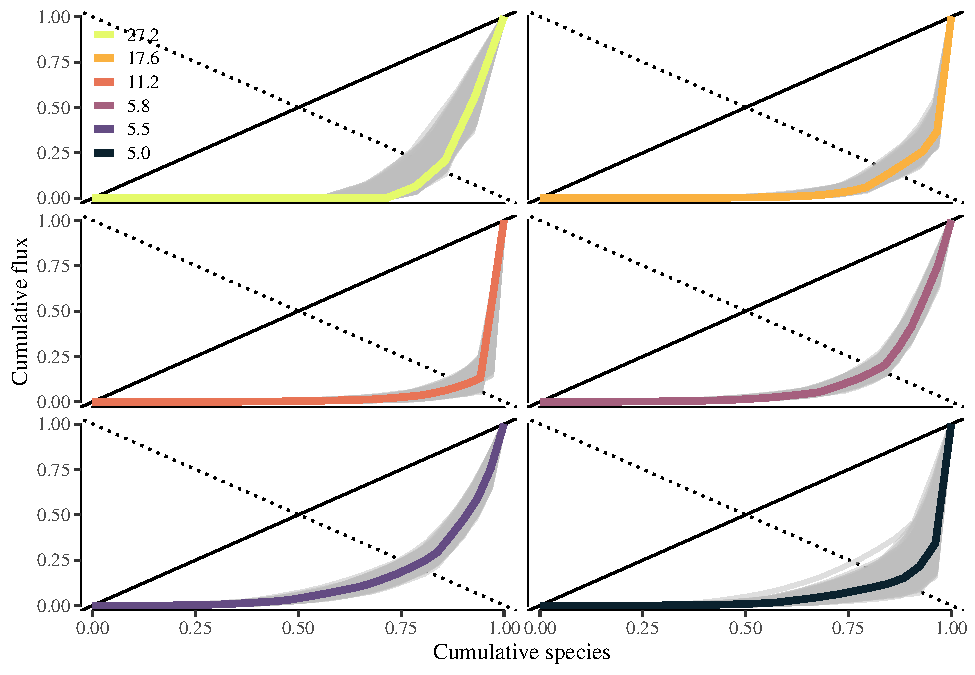
\includegraphics{Junker_temp-energy-flux_appendixS2_files/figure-latex/raw lorenz-1.pdf}
\caption{Appendix S2:Figure S1. Lorenz plot of relative community flux
by species in ascending order of annual population organic matter flux
(g AFDM m\textsuperscript{-2} y\textsuperscript{-1})}
\end{figure}

\newpage

Appendix S2: Figure S2

\begin{figure}
\centering
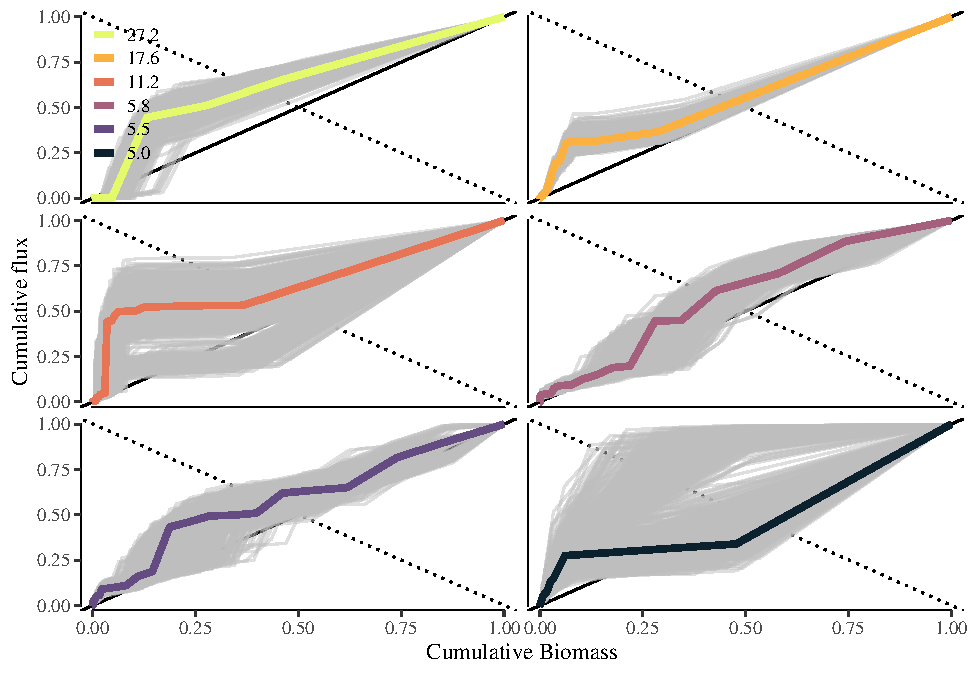
\includegraphics{Junker_temp-energy-flux_appendixS2_files/figure-latex/biomass lorenz-1.pdf}
\caption{Appendix S2:Figure S2. Cumulative plot of relative community
flux by species in relation to mean annual population biomass (mg
m\textsuperscript{-2}).}
\end{figure}

\newpage

Appendix S2: Figure S3

\begin{figure}
\centering
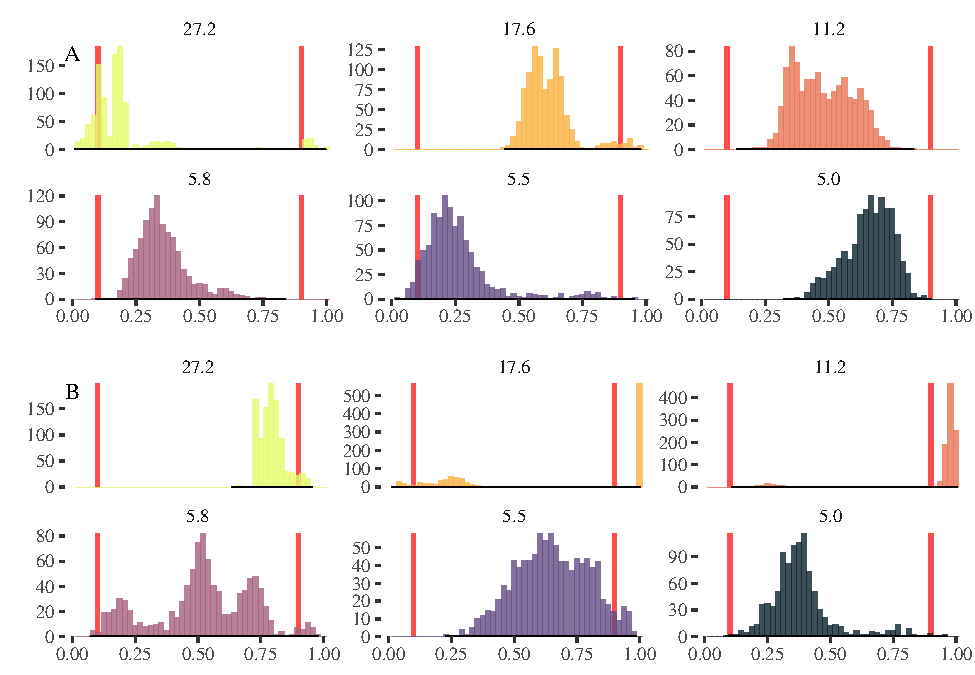
\includegraphics{Junker_temp-energy-flux_appendixS2_files/figure-latex/skew distribution-1.pdf}
\caption{Appendix S2:Figure S3. Probability distribution of empirical
Sk\textsubscript{flux} measurements in relation to (a) mean body size
and (b) annual P:B compared to random species ordering. The red lines
represent the 2.5\% and 97.5\% percentiles of the Sk\textsubscript{flux}
values from random ordering distributions in each stream community.}
\end{figure}

\end{document}
